\documentclass[hyperref=unicode,graphics=pdflatex,13pt]{beamer}

\mode<presentation>
{
  \usetheme{default}
  %\usecolortheme{seahorse}
  \usefonttheme{serif}
  \setbeamercovered{invisible}
  \setbeamertemplate{footline}{\hfill\insertframenumber/\inserttotalframenumber}
    \setbeamersize{text margin left=0.4cm,text margin right=0.4cm, sidebar width left=0cm}
}

\graphicspath{{pic/}}
\usepackage{subfig}
\usepackage[utf8]{inputenc}
\usepackage[T2A]{fontenc}
\usepackage[english,russian]{babel}
\usepackage{times}
\usepackage{float}
\usepackage{color, colortbl}
\usepackage{caption}
\definecolor{res}{RGB}{255, 215, 0}
\definecolor{olivegreen}{RGB}{38, 141, 38}

\definecolor{res2}{RGB}{255,236,139}
\definecolor{res1}{RGB}{255,185,15}
% \definecolor{res2}{RGB}{230,230,230}
% \definecolor{res1}{RGB}{153,149,140}
\definecolor{res3}{RGB}{102,205,0}
\definecolor{res4}{RGB}{152,251,152}
%\usepackage{xcolor}

\beamertemplatenavigationsymbolsempty 

\newcommand\highlight[1]{{\color{blue}{#1}}}
\newcommand\col[1]{{\color{olivegreen}{#1}}}

\title[Адаптивная настройка параметров\ldots]{Адаптивная настройка параметров эволюционных алгоритмов с помощью обучения с подкреплением}

\author[\mbox{А.~Рост}]{Рост Аркадий Юрьевич \\ Научный руководитель~---~д.т.н.,~профессор~А.~А.~Шалыто}
\institute[Университет ИТМО]{
{
\includegraphics[width=0.3\textwidth]{itmo-dots-ru-small.png}}}
\date[]{2015 г.}

\AtBeginSection[] {
  \begin{frame}<beamer>{}
    \tableofcontents[currentsection,currentsubsection]
  \end{frame}
}

\begin{document}

\begin{frame}
  \titlepage
\end{frame}

\begin{frame}{Цели}
    Подбор оптимальных значений параметров ЭА затруднен тем, что они:
    \begin{itemize}
            \item зависят не только от ЭА, но и от экземпляра решаемой задачи;
            \item могут меняться во время работы алгоритма.
    \end{itemize}
    Следовательно, надо выбирать значения параметров во время работы ЭА.
\end{frame}

\begin{frame}{Выбор значения параметра}
    Значения параметра ЭА можно ограничить некоторым интервалом.

    Для дискретизации задачи интервал разбивают на части.
    \begin{itemize}
        \item статически (q-learning)
        \item динамически (arpc, earpc)
    \end{itemize}
\end{frame}

\begin{frame}{Обучение с подкреплением}
    \begin{itemize}
    \item дискретное множество состояний среды \textit{S}
    \item дискретное множество действий агента \textit{A}
    \item функцию награды $R : S \times A \rightarrow \mathbb{R}$
    \item функцию переходов $T : S \times A \times S \rightarrow \mathbb{R}$
    \end{itemize}
\end{frame}

\begin{frame}{Обучение с подкреплением}
    \begin{itemize}
        \item агент выбирает действие --- значения параметров ЭА
        \item среда --- ЭА, формирует следующее поколение
        \item агенту возвращается награда, зависящая от значения функции приспособленности
        \item значение ожидаемой награды $Q(s, a)\gets Q(s,a)+\alpha(r+\gamma\max\limits_{a'}Q(s',a')-Q(s,a))$
    \end{itemize}
\end{frame}

\begin{frame}{Среда}
 Состояние среды описывается:
 \begin{itemize}
     \item значениями параметров $\{p_i\}$
     \item наблюдаемыми характеристиками ЭА $\{o_i\}$, такими как:
     \begin{itemize}
        \item генетическое разнообразие
        \item разнообразие значений функции приспособленности
        \item стагнация
        \item прирост значения функции приспособленности
     \end{itemize}
 \end{itemize}
\end{frame}

\begin{frame} {UTree}
  \begin{itemize}
    \item выделяется набор состояний, в каждом из которых свое распределение вероятностей выбора части интервала значений параметра
    \item состояние выбирается с помощью дерева решений, которое строится во время работы алгоритма
    \item в вершинах дерева стоят условия на наблюдаемые характеристики ЭА
  \end{itemize}
\end{frame}

\begin{frame}{Построение UTree}
    \begin{itemize}
        \item начинаем с одним состоянием
        \item в состоянии запоминаем <I, a, I', r>
        \item $q \gets r + \gamma E(Q(S'))$, где $E(Q(S'))$~--- ожидаемая награда в состоянии $S'$, соответствующее параметрам $I'$
        \item статистический тест Колмогорова-Смирнова
    \end{itemize}
\end{frame}


\begin{frame}{Earpc}
  \begin{itemize}
    \item интервал значений параметра разбивается во время работы на $k$ частей
    \item каждому выбранному значению $p_i$ соответствует $q_i$
    \item разбиваем выбранные значения на $k$ кластеров
    \item ищем разбиение, минимизируя \textit{энтропию}
    \item $Q_{k_j} = \frac{1}{|c(k_j)|}\sum\limits_{p_i \in k_j}{q_i}$
    \item $P_{k_j} \propto Q_{k_j}$
  \end{itemize}
\end{frame}


\begin{frame}{Разрабатываемый метод 1}
    \begin{itemize}
        \item объединяет \textit{UTree} и \textit{Earpc}
        \item динамически разбивает интервал значений параметра
        \item $E(Q) = \sum{P_{k_j}Q_{k_j}}$
    \end{itemize}
\end{frame}

\begin{frame}{Разрабатываемый метод 2}
  \begin{itemize}
   \item одно состояние среды в каждый момент времени
   \item динамически разбивается интервал значений на основе критерия однородности
   \item выбор действия на основе алгоритма \textit{Q}-обучения с $\epsilon$-жадной стратегией исследования среды
  \end{itemize}
\end{frame}

\begin{frame}{Модельная задача}
    \begin{itemize}
        \item найти минимум функции $f(x_1, x_2)$ с заданной точностью $\epsilon$
        \item $R = c(\frac{f_t}{f_{t + 1}} - 1)$
        \item $(\mu+\lambda)$-эволюционная стратегия
        \item мутация $x_i + \sigma \cdot dx_i$, $\sigma \in [0, k]$, $dx_i \sim \mathcal{N}(0,1)$
    \end{itemize}
\end{frame}

\begin{frame}{Значения параметров}
	\begin{itemize}
		 \item $\mu \in \{1, 5, 10\}$
		 \item $\lambda \in \{1, 3, 7\}$
		 \item $\sigma \in \{1, 2, 3\}$
		 \item $\epsilon = 10^{-5}$
	\end{itemize}
\end{frame}

\begin{frame}{Рассматриваемые задачи}
	\begin{itemize}
		\item сфера:  $x_1, x_2 \in [-10; 15]$, $f(x_1, x_2) =x_1^2 + x_2^2$
		\item функция Розенброка: $x_1, x_2 \in [-15; 10]$, 
			\begin{align}
				f(x_1, x_2) = (1 - x_1^2)^2 + 100(x_2 - x_1^2)^2 \nonumber
			\end{align}
		\item функция Леви:  $x, y \in [-10; 10]$
			\begin{align}
				f(x_1, x2) = &sin^2(3\pi x) + (x - 1)^2(1 + sin^2(3\pi y)) + \nonumber\\
				& + (y - 1)^2(1 + sin^2(2\pi y)) \nonumber
			\end{align}
		\item функция Растригина: $x_1, x_2 \in [-5; 5]$,
			\begin{align}
				f(x_1, .., x_n) = An + \sum\limits_{i = 1}^n\left[ x_i^2 - Acos\left(2 \pi x_i \right)\right] \nonumber
			\end{align}
	\end{itemize}
\end{frame}

\begin{frame}{Результаты: adaptive}
	 \begin{figure}
	  \centering
	  \subfloat[График выбранных значений $\sigma$.]{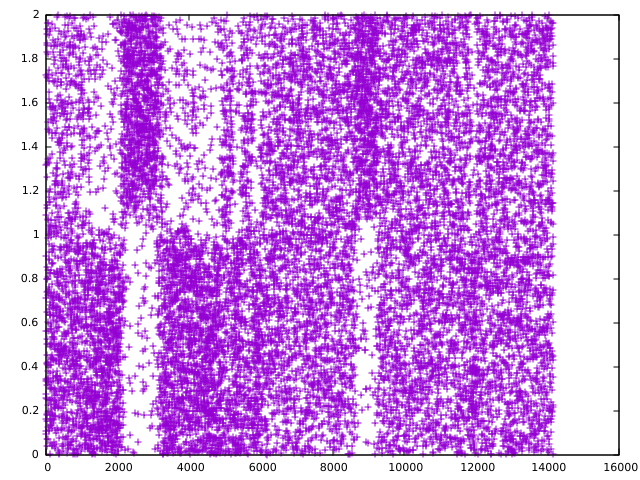
\includegraphics[width=0.5\textwidth]{earpc_sphere_dist.png}}
	  \subfloat[График значения точки разбиения.]{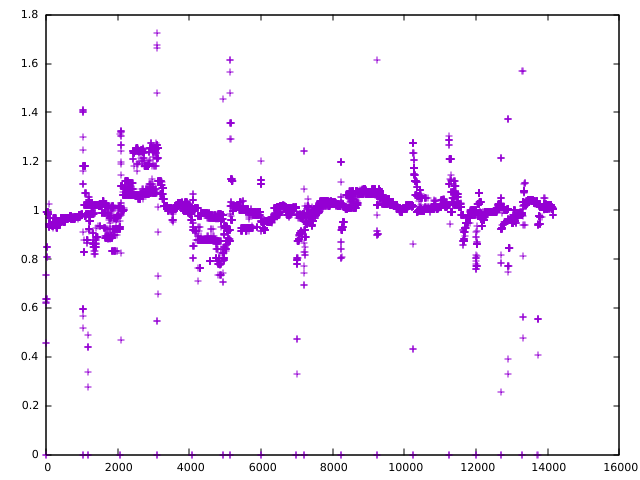
\includegraphics[width=0.5\textwidth]{earpc_sphere.png}}
	  \caption{ Графики работы метода \textit{uarpc}.}
	\end{figure}
\end{frame}

\begin{frame}{Результаты: adaptive}
	\begin{figure}
	  \centering
	  \subfloat[График выбранных значений $\sigma$.]{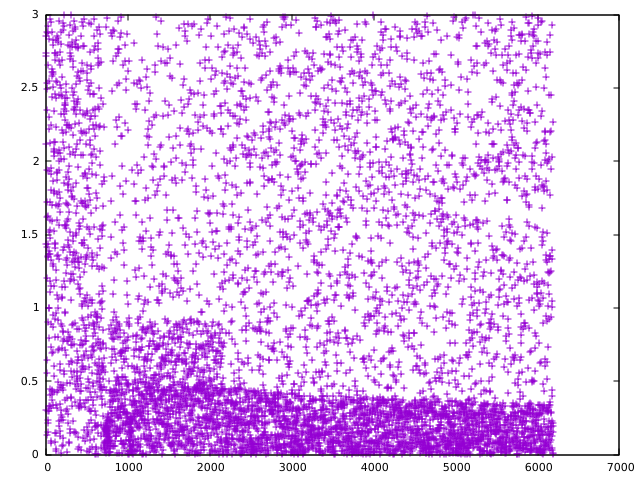
\includegraphics[width=0.5\textwidth]{adaptive_sphere_dist.png}}
	  \subfloat[График значения точек разбиения.]{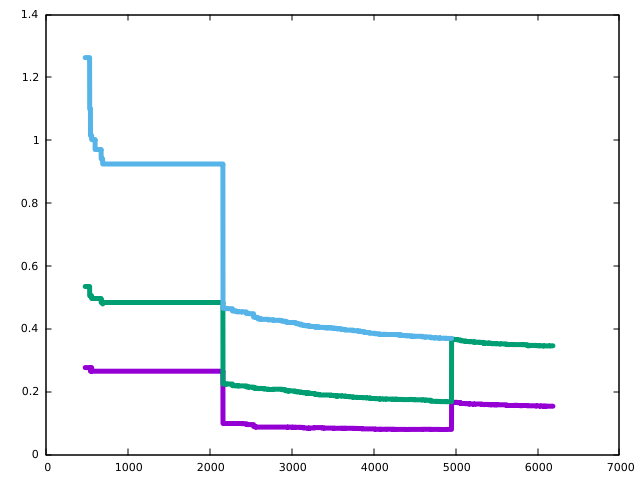
\includegraphics[width=0.5\textwidth]{adaptive_sphere.png}}
	  \caption{ Графики работы метода \textit{adaptive}.}
	\end{figure}
\end{frame}

\begin{frame}{Результаты: karafotias}
	\begin{figure}
	  \centering
	  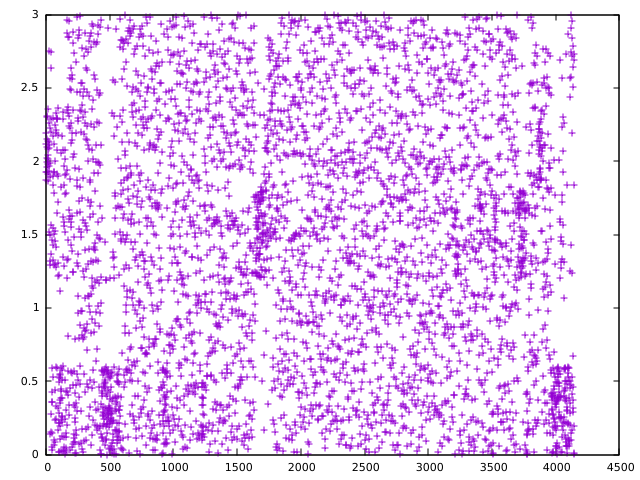
\includegraphics[width=0.5\textwidth]{karafotias_sphere.png}
	  \caption{График выбранных значений $\sigma$ в методе \textit{karafotias}.}
	\end{figure}
\end{frame}

\begin{frame}{Заключение}
    \begin{itemize}
        \item исследованы подходы по настройке параметров ЭА с помощью обучения с подкреплением
        \item предложен способ адаптивного формирования множества действий
        \item предложенный метод успешно протестирован на ряде модельных задач
    \end{itemize}
\end{frame}

\begin{frame}
    \begin{center}
        Спасибо за внимание!
    \end{center}
\end{frame}
\end{document}

